\documentclass[1p]{elsarticle_modified}
%\bibliographystyle{elsarticle-num}

%\usepackage[colorlinks]{hyperref}
%\usepackage{abbrmath_seonhwa} %\Abb, \Ascr, \Acal ,\Abf, \Afrak
\usepackage{amsfonts}
\usepackage{amssymb}
\usepackage{amsmath}
\usepackage{amsthm}
\usepackage{scalefnt}
\usepackage{amsbsy}
\usepackage{kotex}
\usepackage{caption}
\usepackage{subfig}
\usepackage{color}
\usepackage{graphicx}
\usepackage{xcolor} %% white, black, red, green, blue, cyan, magenta, yellow
\usepackage{float}
\usepackage{setspace}
\usepackage{hyperref}

\usepackage{tikz}
\usetikzlibrary{arrows}

\usepackage{multirow}
\usepackage{array} % fixed length table
\usepackage{hhline}

%%%%%%%%%%%%%%%%%%%%%
\makeatletter
\renewcommand*\env@matrix[1][\arraystretch]{%
	\edef\arraystretch{#1}%
	\hskip -\arraycolsep
	\let\@ifnextchar\new@ifnextchar
	\array{*\c@MaxMatrixCols c}}
\makeatother %https://tex.stackexchange.com/questions/14071/how-can-i-increase-the-line-spacing-in-a-matrix
%%%%%%%%%%%%%%%

\usepackage[normalem]{ulem}

\newcommand{\msout}[1]{\ifmmode\text{\sout{\ensuremath{#1}}}\else\sout{#1}\fi}
%SOURCE: \msout is \stkout macro in https://tex.stackexchange.com/questions/20609/strikeout-in-math-mode

\newcommand{\cancel}[1]{
	\ifmmode
	{\color{red}\msout{#1}}
	\else
	{\color{red}\sout{#1}}
	\fi
}

\newcommand{\add}[1]{
	{\color{blue}\uwave{#1}}
}

\newcommand{\replace}[2]{
	\ifmmode
	{\color{red}\msout{#1}}{\color{blue}\uwave{#2}}
	\else
	{\color{red}\sout{#1}}{\color{blue}\uwave{#2}}
	\fi
}

\newcommand{\Sol}{\mathcal{S}} %segment
\newcommand{\D}{D} %diagram
\newcommand{\A}{\mathcal{A}} %arc


%%%%%%%%%%%%%%%%%%%%%%%%%%%%%5 test

\def\sl{\operatorname{\textup{SL}}(2,\Cbb)}
\def\psl{\operatorname{\textup{PSL}}(2,\Cbb)}
\def\quan{\mkern 1mu \triangleright \mkern 1mu}

\theoremstyle{definition}
\newtheorem{thm}{Theorem}[section]
\newtheorem{prop}[thm]{Proposition}
\newtheorem{lem}[thm]{Lemma}
\newtheorem{ques}[thm]{Question}
\newtheorem{cor}[thm]{Corollary}
\newtheorem{defn}[thm]{Definition}
\newtheorem{exam}[thm]{Example}
\newtheorem{rmk}[thm]{Remark}
\newtheorem{alg}[thm]{Algorithm}

\newcommand{\I}{\sqrt{-1}}
\begin{document}

%\begin{frontmatter}
%
%\title{Boundary parabolic representations of knots up to 8 crossings}
%
%%% Group authors per affiliation:
%\author{Yunhi Cho} 
%\address{Department of Mathematics, University of Seoul, Seoul, Korea}
%\ead{yhcho@uos.ac.kr}
%
%
%\author{Seonhwa Kim} %\fnref{s_kim}}
%\address{Center for Geometry and Physics, Institute for Basic Science, Pohang, 37673, Korea}
%\ead{ryeona17@ibs.re.kr}
%
%\author{Hyuk Kim}
%\address{Department of Mathematical Sciences, Seoul National University, Seoul 08826, Korea}
%\ead{hyukkim@snu.ac.kr}
%
%\author{Seokbeom Yoon}
%\address{Department of Mathematical Sciences, Seoul National University, Seoul, 08826,  Korea}
%\ead{sbyoon15@snu.ac.kr}
%
%\begin{abstract}
%We find all boundary parabolic representation of knots up to 8 crossings.
%
%\end{abstract}
%\begin{keyword}
%    \MSC[2010] 57M25 
%\end{keyword}
%
%\end{frontmatter}

%\linenumbers
%\tableofcontents
%
\newcommand\colored[1]{\textcolor{white}{\rule[-0.35ex]{0.8em}{1.4ex}}\kern-0.8em\color{red} #1}%
%\newcommand\colored[1]{\textcolor{white}{ #1}\kern-2.17ex	\textcolor{white}{ #1}\kern-1.81ex	\textcolor{white}{ #1}\kern-2.15ex\color{red}#1	}

{\Large $\underline{12a_{1228}~(K12a_{1228})}$}

\setlength{\tabcolsep}{10pt}
\renewcommand{\arraystretch}{1.6}
\vspace{1cm}\begin{tabular}{m{100pt}>{\centering\arraybackslash}m{274pt}}
\multirow{5}{120pt}{
	\centering
	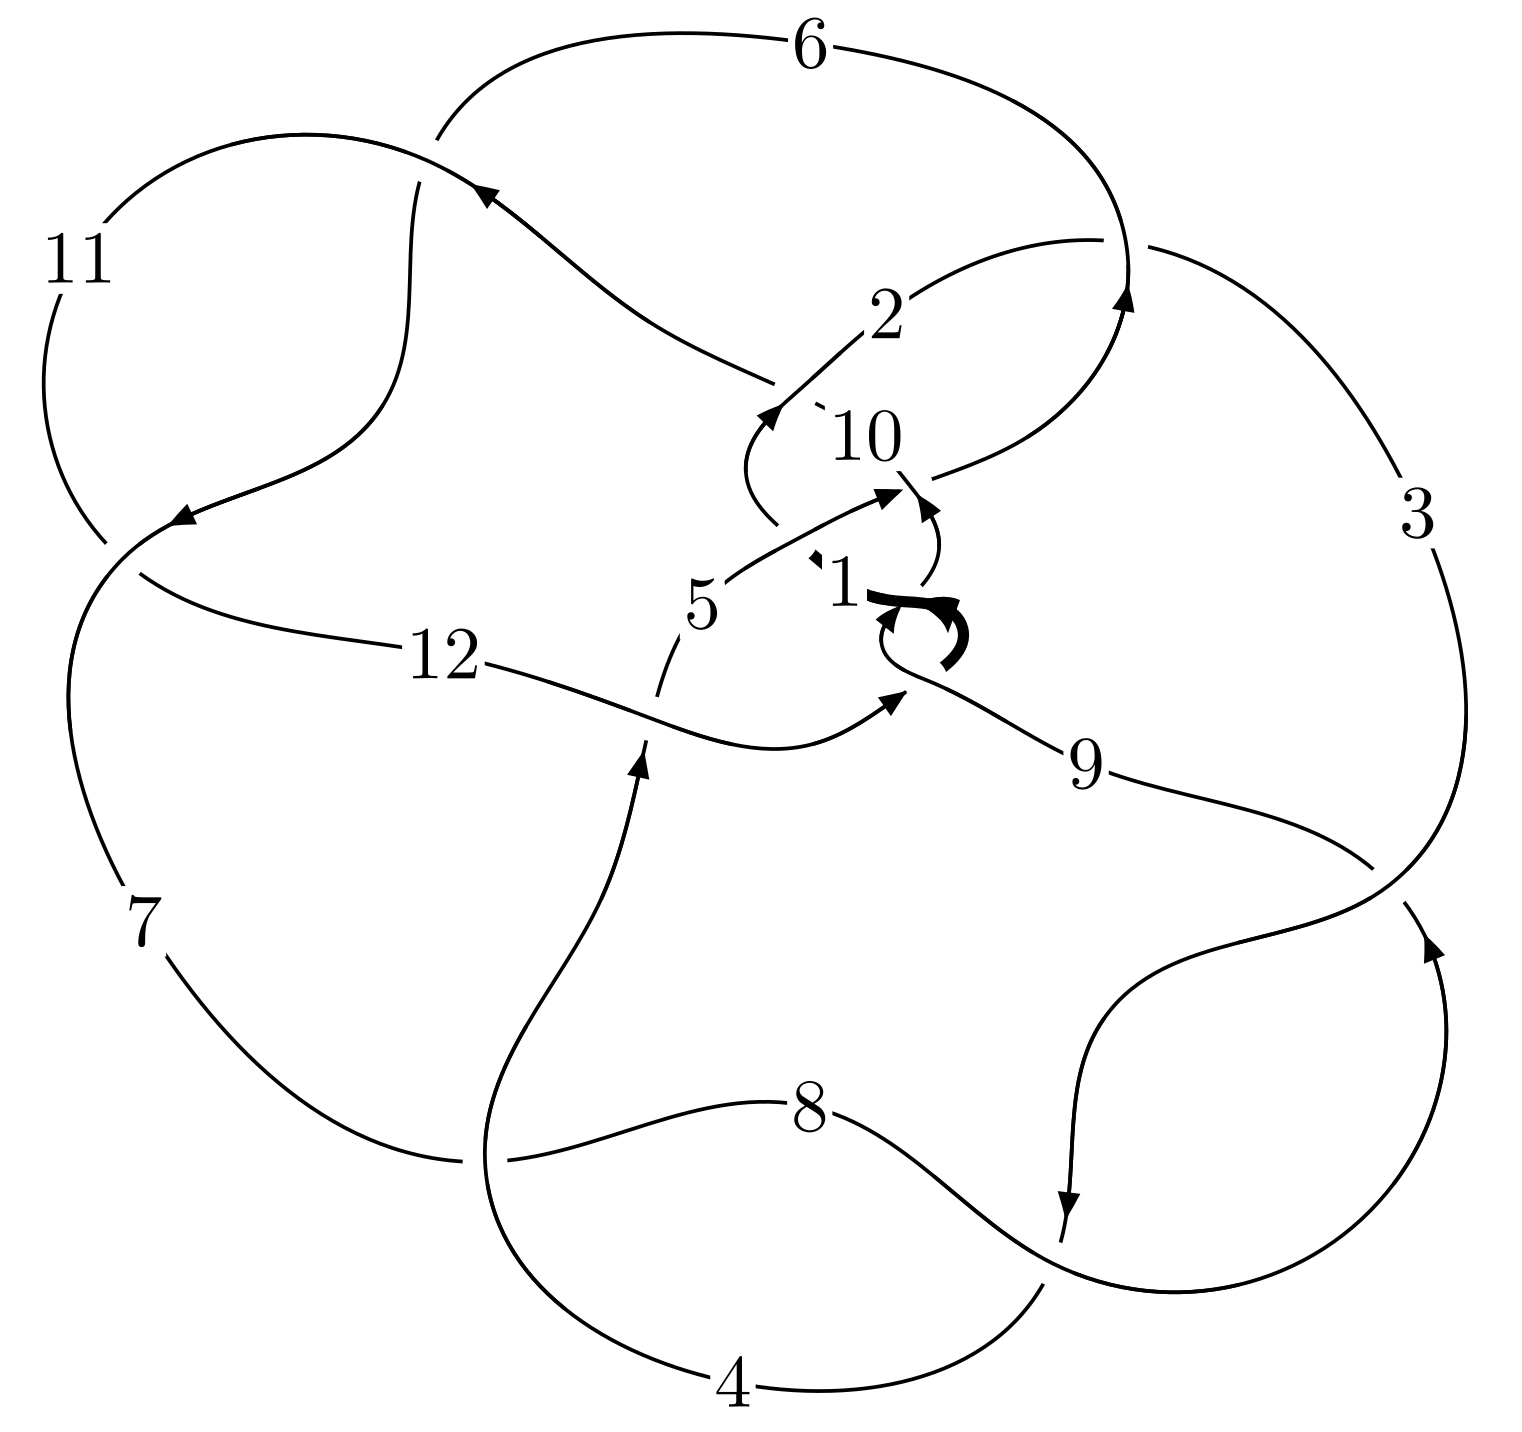
\includegraphics[width=112pt]{../../../GIT/diagram.site/Diagrams/png/2029_12a_1228.png}\\
\ \ \ A knot diagram\footnotemark}&
\allowdisplaybreaks
\textbf{Linearized knot diagam} \\
\cline{2-2}
 &
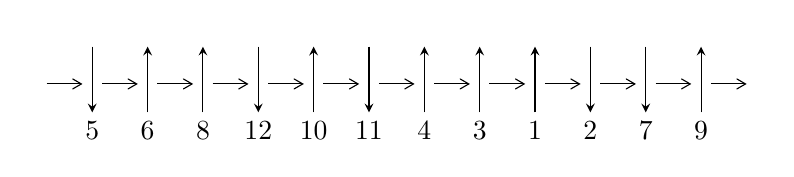
\begin{tikzpicture}[x=20pt, y=17pt]
	% nodes
	\node (C0) at (0, 0) {};
	\node (C1) at (1, 0) {};
	\node (C1U) at (1, +1) {};
	\node (C1D) at (1, -1) {5};

	\node (C2) at (2, 0) {};
	\node (C2U) at (2, +1) {};
	\node (C2D) at (2, -1) {6};

	\node (C3) at (3, 0) {};
	\node (C3U) at (3, +1) {};
	\node (C3D) at (3, -1) {8};

	\node (C4) at (4, 0) {};
	\node (C4U) at (4, +1) {};
	\node (C4D) at (4, -1) {12};

	\node (C5) at (5, 0) {};
	\node (C5U) at (5, +1) {};
	\node (C5D) at (5, -1) {10};

	\node (C6) at (6, 0) {};
	\node (C6U) at (6, +1) {};
	\node (C6D) at (6, -1) {11};

	\node (C7) at (7, 0) {};
	\node (C7U) at (7, +1) {};
	\node (C7D) at (7, -1) {4};

	\node (C8) at (8, 0) {};
	\node (C8U) at (8, +1) {};
	\node (C8D) at (8, -1) {3};

	\node (C9) at (9, 0) {};
	\node (C9U) at (9, +1) {};
	\node (C9D) at (9, -1) {1};

	\node (C10) at (10, 0) {};
	\node (C10U) at (10, +1) {};
	\node (C10D) at (10, -1) {2};

	\node (C11) at (11, 0) {};
	\node (C11U) at (11, +1) {};
	\node (C11D) at (11, -1) {7};

	\node (C12) at (12, 0) {};
	\node (C12U) at (12, +1) {};
	\node (C12D) at (12, -1) {9};
	\node (C13) at (13, 0) {};

	% arrows
	\draw[->,>={angle 60}]
	(C0) edge (C1) (C1) edge (C2) (C2) edge (C3) (C3) edge (C4) (C4) edge (C5) (C5) edge (C6) (C6) edge (C7) (C7) edge (C8) (C8) edge (C9) (C9) edge (C10) (C10) edge (C11) (C11) edge (C12) (C12) edge (C13) ;	\draw[->,>=stealth]
	(C1U) edge (C1D) (C2D) edge (C2U) (C3D) edge (C3U) (C4U) edge (C4D) (C5D) edge (C5U) (C6U) edge (C6D) (C7D) edge (C7U) (C8D) edge (C8U) (C9D) edge (C9U) (C10U) edge (C10D) (C11U) edge (C11D) (C12D) edge (C12U) ;
	\end{tikzpicture} \\
\hhline{~~} \\& 
\textbf{Solving Sequence} \\ \cline{2-2} 
 &
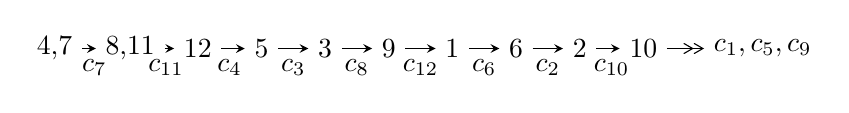
\begin{tikzpicture}[x=23pt, y=7pt]
	% node
	\node (A0) at (-1/8, 0) {4,7};
	\node (A1) at (17/16, 0) {8,11};
	\node (A2) at (17/8, 0) {12};
	\node (A3) at (25/8, 0) {5};
	\node (A4) at (33/8, 0) {3};
	\node (A5) at (41/8, 0) {9};
	\node (A6) at (49/8, 0) {1};
	\node (A7) at (57/8, 0) {6};
	\node (A8) at (65/8, 0) {2};
	\node (A9) at (73/8, 0) {10};
	\node (C1) at (1/2, -1) {$c_{7}$};
	\node (C2) at (13/8, -1) {$c_{11}$};
	\node (C3) at (21/8, -1) {$c_{4}$};
	\node (C4) at (29/8, -1) {$c_{3}$};
	\node (C5) at (37/8, -1) {$c_{8}$};
	\node (C6) at (45/8, -1) {$c_{12}$};
	\node (C7) at (53/8, -1) {$c_{6}$};
	\node (C8) at (61/8, -1) {$c_{2}$};
	\node (C9) at (69/8, -1) {$c_{10}$};
	\node (A10) at (11, 0) {$c_{1},c_{5},c_{9}$};

	% edge
	\draw[->,>=stealth]	
	(A0) edge (A1) (A1) edge (A2) (A2) edge (A3) (A3) edge (A4) (A4) edge (A5) (A5) edge (A6) (A6) edge (A7) (A7) edge (A8) (A8) edge (A9) ;
	\draw[->>,>={angle 60}]	
	(A9) edge (A10);
\end{tikzpicture} \\ 

\end{tabular} \\

\footnotetext{
The image of knot diagram is generated by the software ``\textbf{Draw programme}" developed by Andrew Bartholomew(\url{http://www.layer8.co.uk/maths/draw/index.htm\#Running-draw}), where we modified some parts for our purpose(\url{https://github.com/CATsTAILs/LinksPainter}).
}\phantom \\ \newline 
\centering \textbf{Ideals for irreducible components\footnotemark of $X_{\text{par}}$} 
 
\begin{align*}
I^u_{1}&=\langle 
-6.01811\times10^{386} u^{129}-3.95810\times10^{385} u^{128}+\cdots+1.46054\times10^{387} b-5.70213\times10^{386},\\
\phantom{I^u_{1}}&\phantom{= \langle  }1.81978\times10^{387} u^{129}+1.68335\times10^{386} u^{128}+\cdots+1.46054\times10^{387} a-7.47460\times10^{388},\\
\phantom{I^u_{1}}&\phantom{= \langle  }u^{130}+65 u^{128}+\cdots+25 u+1\rangle \\
I^u_{2}&=\langle 
2337 u^{31}-6 u^{30}+\cdots+631 b+5039,\;1267570 u^{31}+992573 u^{30}+\cdots+239149 a+339493,\\
\phantom{I^u_{2}}&\phantom{= \langle  }u^{32}+u^{31}+\cdots+4 u-1\rangle \\
\\
\end{align*}
\raggedright * 2 irreducible components of $\dim_{\mathbb{C}}=0$, with total 162 representations.\\
\footnotetext{All coefficients of polynomials are rational numbers. But the coefficients are sometimes approximated in decimal forms when there is not enough margin.}
\newpage
\renewcommand{\arraystretch}{1}
\centering \section*{I. $I^u_{1}= \langle -6.02\times10^{386} u^{129}-3.96\times10^{385} u^{128}+\cdots+1.46\times10^{387} b-5.70\times10^{386},\;1.82\times10^{387} u^{129}+1.68\times10^{386} u^{128}+\cdots+1.46\times10^{387} a-7.47\times10^{388},\;u^{130}+65 u^{128}+\cdots+25 u+1 \rangle$}
\flushleft \textbf{(i) Arc colorings}\\
\begin{tabular}{m{7pt} m{180pt} m{7pt} m{180pt} }
\flushright $a_{4}=$&$\begin{pmatrix}0\\u\end{pmatrix}$ \\
\flushright $a_{7}=$&$\begin{pmatrix}1\\0\end{pmatrix}$ \\
\flushright $a_{8}=$&$\begin{pmatrix}1\\- u^2\end{pmatrix}$ \\
\flushright $a_{11}=$&$\begin{pmatrix}-1.24596 u^{129}-0.115255 u^{128}+\cdots+72.2066 u+51.1769\\0.412047 u^{129}+0.0271002 u^{128}+\cdots-33.1795 u+0.390412\end{pmatrix}$ \\
\flushright $a_{12}=$&$\begin{pmatrix}-1.65801 u^{129}-0.142356 u^{128}+\cdots+105.386 u+50.7865\\0.412047 u^{129}+0.0271002 u^{128}+\cdots-33.1795 u+0.390412\end{pmatrix}$ \\
\flushright $a_{5}=$&$\begin{pmatrix}2.49008 u^{129}+1.08728 u^{128}+\cdots-622.790 u+26.2361\\0.690479 u^{129}+0.332737 u^{128}+\cdots-117.082 u-2.07945\end{pmatrix}$ \\
\flushright $a_{3}=$&$\begin{pmatrix}- u\\u^3+u\end{pmatrix}$ \\
\flushright $a_{9}=$&$\begin{pmatrix}u^2+1\\- u^4-2 u^2\end{pmatrix}$ \\
\flushright $a_{1}=$&$\begin{pmatrix}-1.17148 u^{129}-0.0845750 u^{128}+\cdots+93.0440 u+51.8431\\0.316454 u^{129}+0.174664 u^{128}+\cdots-29.3185 u+0.537108\end{pmatrix}$ \\
\flushright $a_{6}=$&$\begin{pmatrix}1.66777 u^{129}+0.545132 u^{128}+\cdots+118.027 u-65.5786\\-0.411679 u^{129}-0.145347 u^{128}+\cdots+52.8301 u-0.482638\end{pmatrix}$ \\
\flushright $a_{2}=$&$\begin{pmatrix}7.00138 u^{129}+0.814010 u^{128}+\cdots-2243.97 u+34.5505\\-0.0796178 u^{129}+0.188534 u^{128}+\cdots-79.5670 u+1.05186\end{pmatrix}$ \\
\flushright $a_{10}=$&$\begin{pmatrix}4.05410 u^{129}+0.547154 u^{128}+\cdots-65.5783 u-74.4592\\-0.0343714 u^{129}+0.0978812 u^{128}+\cdots+30.9080 u-1.20261\end{pmatrix}$\\&\end{tabular}
\flushleft \textbf{(ii) Obstruction class $= -1$}\\~\\
\flushleft \textbf{(iii) Cusp Shapes $= 2.01406 u^{129}+0.00528034 u^{128}+\cdots-230.499 u-15.4118$}\\~\\
\newpage\renewcommand{\arraystretch}{1}
\flushleft \textbf{(iv) u-Polynomials at the component}\newline \\
\begin{tabular}{m{50pt}|m{274pt}}
Crossings & \hspace{64pt}u-Polynomials at each crossing \\
\hline $$\begin{aligned}c_{1}\end{aligned}$$&$\begin{aligned}
&u^{130}+u^{129}+\cdots+4 u+1
\end{aligned}$\\
\hline $$\begin{aligned}c_{2}\end{aligned}$$&$\begin{aligned}
&u^{130}+3 u^{129}+\cdots+11268 u+1367
\end{aligned}$\\
\hline $$\begin{aligned}c_{3},c_{7},c_{8}\end{aligned}$$&$\begin{aligned}
&u^{130}+65 u^{128}+\cdots-25 u+1
\end{aligned}$\\
\hline $$\begin{aligned}c_{4}\end{aligned}$$&$\begin{aligned}
&u^{130}-20 u^{128}+\cdots+4232509101 u+1162172247
\end{aligned}$\\
\hline $$\begin{aligned}c_{5}\end{aligned}$$&$\begin{aligned}
&u^{130}+3 u^{129}+\cdots-4845 u-2433
\end{aligned}$\\
\hline $$\begin{aligned}c_{6},c_{11}\end{aligned}$$&$\begin{aligned}
&u^{130}- u^{129}+\cdots+20276 u-12013
\end{aligned}$\\
\hline $$\begin{aligned}c_{9},c_{12}\end{aligned}$$&$\begin{aligned}
&u^{130}- u^{129}+\cdots+72388 u-2507
\end{aligned}$\\
\hline $$\begin{aligned}c_{10}\end{aligned}$$&$\begin{aligned}
&u^{130}+7 u^{129}+\cdots-3637 u-1103
\end{aligned}$\\
\hline
\end{tabular}\\~\\
\newpage\renewcommand{\arraystretch}{1}
\flushleft \textbf{(v) Riley Polynomials at the component}\newline \\
\begin{tabular}{m{50pt}|m{274pt}}
Crossings & \hspace{64pt}Riley Polynomials at each crossing \\
\hline $$\begin{aligned}c_{1}\end{aligned}$$&$\begin{aligned}
&y^{130}+21 y^{129}+\cdots-332 y+1
\end{aligned}$\\
\hline $$\begin{aligned}c_{2}\end{aligned}$$&$\begin{aligned}
&y^{130}+27 y^{129}+\cdots+8414388 y+1868689
\end{aligned}$\\
\hline $$\begin{aligned}c_{3},c_{7},c_{8}\end{aligned}$$&$\begin{aligned}
&y^{130}+130 y^{129}+\cdots-2035 y+1
\end{aligned}$\\
\hline $$\begin{aligned}c_{4}\end{aligned}$$&$\begin{aligned}
&y^{130}-40 y^{129}+\cdots-4.82\times10^{19} y+1.35\times10^{18}
\end{aligned}$\\
\hline $$\begin{aligned}c_{5}\end{aligned}$$&$\begin{aligned}
&y^{130}-27 y^{129}+\cdots-381850059 y+5919489
\end{aligned}$\\
\hline $$\begin{aligned}c_{6},c_{11}\end{aligned}$$&$\begin{aligned}
&y^{130}-109 y^{129}+\cdots+3652617438 y+144312169
\end{aligned}$\\
\hline $$\begin{aligned}c_{9},c_{12}\end{aligned}$$&$\begin{aligned}
&y^{130}-89 y^{129}+\cdots-1089734184 y+6285049
\end{aligned}$\\
\hline $$\begin{aligned}c_{10}\end{aligned}$$&$\begin{aligned}
&y^{130}-25 y^{129}+\cdots-58049277 y+1216609
\end{aligned}$\\
\hline
\end{tabular}\\~\\
\newpage\flushleft \textbf{(vi) Complex Volumes and Cusp Shapes}
$$\begin{array}{c|c|c}  
\text{Solutions to }I^u_{1}& \I (\text{vol} + \sqrt{-1}CS) & \text{Cusp shape}\\
 \hline 
\begin{aligned}
u &= -0.878351 + 0.479501 I \\
a &= \phantom{-}0.267905 - 0.715082 I \\
b &= \phantom{-}1.265230 - 0.145494 I\end{aligned}
 & -4.46528 + 3.18471 I & \phantom{-0.000000 } 0 \\ \hline\begin{aligned}
u &= -0.878351 - 0.479501 I \\
a &= \phantom{-}0.267905 + 0.715082 I \\
b &= \phantom{-}1.265230 + 0.145494 I\end{aligned}
 & -4.46528 - 3.18471 I & \phantom{-0.000000 } 0 \\ \hline\begin{aligned}
u &= -0.904178 + 0.479209 I \\
a &= \phantom{-}0.677224 - 0.825676 I \\
b &= \phantom{-}1.42958 + 0.41209 I\end{aligned}
 & -0.7984 - 14.1663 I & \phantom{-0.000000 } 0 \\ \hline\begin{aligned}
u &= -0.904178 - 0.479209 I \\
a &= \phantom{-}0.677224 + 0.825676 I \\
b &= \phantom{-}1.42958 - 0.41209 I\end{aligned}
 & -0.7984 + 14.1663 I & \phantom{-0.000000 } 0 \\ \hline\begin{aligned}
u &= -0.597787 + 0.841552 I \\
a &= -0.603320 + 0.306989 I \\
b &= -0.114008 - 0.193764 I\end{aligned}
 & \phantom{-}2.91845 - 3.75419 I & \phantom{-0.000000 } 0 \\ \hline\begin{aligned}
u &= -0.597787 - 0.841552 I \\
a &= -0.603320 - 0.306989 I \\
b &= -0.114008 + 0.193764 I\end{aligned}
 & \phantom{-}2.91845 + 3.75419 I & \phantom{-0.000000 } 0 \\ \hline\begin{aligned}
u &= -0.724677 + 0.634607 I \\
a &= -0.768164 + 0.720424 I \\
b &= -1.37841 - 0.37858 I\end{aligned}
 & -5.07932 - 8.49653 I & \phantom{-0.000000 } 0 \\ \hline\begin{aligned}
u &= -0.724677 - 0.634607 I \\
a &= -0.768164 - 0.720424 I \\
b &= -1.37841 + 0.37858 I\end{aligned}
 & -5.07932 + 8.49653 I & \phantom{-0.000000 } 0 \\ \hline\begin{aligned}
u &= -0.982121 + 0.472548 I \\
a &= -0.484899 + 0.576892 I \\
b &= -1.183440 - 0.246868 I\end{aligned}
 & \phantom{-}1.58463 - 5.74871 I & \phantom{-0.000000 } 0 \\ \hline\begin{aligned}
u &= -0.982121 - 0.472548 I \\
a &= -0.484899 - 0.576892 I \\
b &= -1.183440 + 0.246868 I\end{aligned}
 & \phantom{-}1.58463 + 5.74871 I & \phantom{-0.000000 } 0\\
 \hline 
 \end{array}$$\newpage$$\begin{array}{c|c|c}  
\text{Solutions to }I^u_{1}& \I (\text{vol} + \sqrt{-1}CS) & \text{Cusp shape}\\
 \hline 
\begin{aligned}
u &= \phantom{-}0.615550 + 0.655227 I \\
a &= \phantom{-}1.23994 + 1.59607 I \\
b &= \phantom{-}1.248160 - 0.021656 I\end{aligned}
 & -1.13752 + 4.31310 I & \phantom{-0.000000 } 0 \\ \hline\begin{aligned}
u &= \phantom{-}0.615550 - 0.655227 I \\
a &= \phantom{-}1.23994 - 1.59607 I \\
b &= \phantom{-}1.248160 + 0.021656 I\end{aligned}
 & -1.13752 - 4.31310 I & \phantom{-0.000000 } 0 \\ \hline\begin{aligned}
u &= \phantom{-}0.385384 + 0.792448 I \\
a &= -1.231870 + 0.402891 I \\
b &= \phantom{-}0.105055 + 0.547279 I\end{aligned}
 & \phantom{-}3.03102 - 5.24392 I & \phantom{-0.000000 } 0 \\ \hline\begin{aligned}
u &= \phantom{-}0.385384 - 0.792448 I \\
a &= -1.231870 - 0.402891 I \\
b &= \phantom{-}0.105055 - 0.547279 I\end{aligned}
 & \phantom{-}3.03102 + 5.24392 I & \phantom{-0.000000 } 0 \\ \hline\begin{aligned}
u &= -0.818503 + 0.290253 I \\
a &= \phantom{-}0.142451 + 0.334207 I \\
b &= -0.086924 - 0.484757 I\end{aligned}
 & \phantom{-}4.56441 - 1.19346 I & \phantom{-0.000000 } 0 \\ \hline\begin{aligned}
u &= -0.818503 - 0.290253 I \\
a &= \phantom{-}0.142451 - 0.334207 I \\
b &= -0.086924 + 0.484757 I\end{aligned}
 & \phantom{-}4.56441 + 1.19346 I & \phantom{-0.000000 } 0 \\ \hline\begin{aligned}
u &= -0.820647 + 0.789678 I \\
a &= -0.634880 + 0.632957 I \\
b &= -1.350430 + 0.261267 I\end{aligned}
 & -1.65517 + 8.35247 I & \phantom{-0.000000 } 0 \\ \hline\begin{aligned}
u &= -0.820647 - 0.789678 I \\
a &= -0.634880 - 0.632957 I \\
b &= -1.350430 - 0.261267 I\end{aligned}
 & -1.65517 - 8.35247 I & \phantom{-0.000000 } 0 \\ \hline\begin{aligned}
u &= \phantom{-}0.386861 + 1.075540 I \\
a &= \phantom{-}1.351750 - 0.141898 I \\
b &= \phantom{-}0.493213 - 0.154400 I\end{aligned}
 & \phantom{-}2.20870 + 1.30818 I & \phantom{-0.000000 } 0 \\ \hline\begin{aligned}
u &= \phantom{-}0.386861 - 1.075540 I \\
a &= \phantom{-}1.351750 + 0.141898 I \\
b &= \phantom{-}0.493213 + 0.154400 I\end{aligned}
 & \phantom{-}2.20870 - 1.30818 I & \phantom{-0.000000 } 0\\
 \hline 
 \end{array}$$\newpage$$\begin{array}{c|c|c}  
\text{Solutions to }I^u_{1}& \I (\text{vol} + \sqrt{-1}CS) & \text{Cusp shape}\\
 \hline 
\begin{aligned}
u &= \phantom{-}0.712561 + 0.448408 I \\
a &= -0.63173 - 1.27602 I \\
b &= -1.338250 + 0.447663 I\end{aligned}
 & -2.99150 + 6.35567 I & \phantom{-0.000000 } 0 \\ \hline\begin{aligned}
u &= \phantom{-}0.712561 - 0.448408 I \\
a &= -0.63173 + 1.27602 I \\
b &= -1.338250 - 0.447663 I\end{aligned}
 & -2.99150 - 6.35567 I & \phantom{-0.000000 } 0 \\ \hline\begin{aligned}
u &= \phantom{-}0.829587\phantom{ +0.000000I} \\
a &= \phantom{-}0.323136\phantom{ +0.000000I} \\
b &= -1.48778\phantom{ +0.000000I}\end{aligned}
 & -4.55769\phantom{ +0.000000I} & \phantom{-0.000000 } 0 \\ \hline\begin{aligned}
u &= \phantom{-}0.646603 + 0.513783 I \\
a &= \phantom{-}0.371738 + 0.586985 I \\
b &= \phantom{-}1.289990 + 0.231810 I\end{aligned}
 & -3.27855 - 1.86425 I & \phantom{-0.000000 } 0 \\ \hline\begin{aligned}
u &= \phantom{-}0.646603 - 0.513783 I \\
a &= \phantom{-}0.371738 - 0.586985 I \\
b &= \phantom{-}1.289990 - 0.231810 I\end{aligned}
 & -3.27855 + 1.86425 I & \phantom{-0.000000 } 0 \\ \hline\begin{aligned}
u &= \phantom{-}1.033090 + 0.570815 I \\
a &= \phantom{-}0.853456 + 0.628055 I \\
b &= \phantom{-}1.306130 - 0.156354 I\end{aligned}
 & \phantom{-}0.26850 + 3.54378 I & \phantom{-0.000000 } 0 \\ \hline\begin{aligned}
u &= \phantom{-}1.033090 - 0.570815 I \\
a &= \phantom{-}0.853456 - 0.628055 I \\
b &= \phantom{-}1.306130 + 0.156354 I\end{aligned}
 & \phantom{-}0.26850 - 3.54378 I & \phantom{-0.000000 } 0 \\ \hline\begin{aligned}
u &= -0.782500 + 0.949740 I \\
a &= \phantom{-}0.676862 - 0.554508 I \\
b &= \phantom{-}1.124950 - 0.039839 I\end{aligned}
 & \phantom{-}0.214016 - 0.410424 I & \phantom{-0.000000 } 0 \\ \hline\begin{aligned}
u &= -0.782500 - 0.949740 I \\
a &= \phantom{-}0.676862 + 0.554508 I \\
b &= \phantom{-}1.124950 + 0.039839 I\end{aligned}
 & \phantom{-}0.214016 + 0.410424 I & \phantom{-0.000000 } 0 \\ \hline\begin{aligned}
u &= -0.765551\phantom{ +0.000000I} \\
a &= \phantom{-}0.996922\phantom{ +0.000000I} \\
b &= -1.07406\phantom{ +0.000000I}\end{aligned}
 & \phantom{-}2.38604\phantom{ +0.000000I} & \phantom{-0.000000 } 0\\
 \hline 
 \end{array}$$\newpage$$\begin{array}{c|c|c}  
\text{Solutions to }I^u_{1}& \I (\text{vol} + \sqrt{-1}CS) & \text{Cusp shape}\\
 \hline 
\begin{aligned}
u &= -0.293830 + 1.202900 I \\
a &= \phantom{-}0.267092 - 0.713391 I \\
b &= \phantom{-}1.032950 + 0.235404 I\end{aligned}
 & -1.28452 - 3.87204 I & \phantom{-0.000000 } 0 \\ \hline\begin{aligned}
u &= -0.293830 - 1.202900 I \\
a &= \phantom{-}0.267092 + 0.713391 I \\
b &= \phantom{-}1.032950 - 0.235404 I\end{aligned}
 & -1.28452 + 3.87204 I & \phantom{-0.000000 } 0 \\ \hline\begin{aligned}
u &= \phantom{-}0.755209\phantom{ +0.000000I} \\
a &= -0.818690\phantom{ +0.000000I} \\
b &= -1.40811\phantom{ +0.000000I}\end{aligned}
 & \phantom{-}0.825266\phantom{ +0.000000I} & \phantom{-0.000000 } 0 \\ \hline\begin{aligned}
u &= -0.172994 + 1.236950 I \\
a &= \phantom{-}1.010490 + 0.983822 I \\
b &= -0.553804 + 0.385324 I\end{aligned}
 & -0.29613 - 4.62984 I & \phantom{-0.000000 } 0 \\ \hline\begin{aligned}
u &= -0.172994 - 1.236950 I \\
a &= \phantom{-}1.010490 - 0.983822 I \\
b &= -0.553804 - 0.385324 I\end{aligned}
 & -0.29613 + 4.62984 I & \phantom{-0.000000 } 0 \\ \hline\begin{aligned}
u &= \phantom{-}0.680901 + 0.316640 I \\
a &= \phantom{-}0.043183 - 0.636995 I \\
b &= -0.240222 + 0.999581 I\end{aligned}
 & \phantom{-}4.48026 + 9.15437 I & \phantom{-0.000000 } 0 \\ \hline\begin{aligned}
u &= \phantom{-}0.680901 - 0.316640 I \\
a &= \phantom{-}0.043183 + 0.636995 I \\
b &= -0.240222 - 0.999581 I\end{aligned}
 & \phantom{-}4.48026 - 9.15437 I & \phantom{-0.000000 } 0 \\ \hline\begin{aligned}
u &= \phantom{-}0.907749 + 0.880383 I \\
a &= -0.931871 - 0.374887 I \\
b &= -1.262540 - 0.007209 I\end{aligned}
 & -0.55631 + 3.09812 I & \phantom{-0.000000 } 0 \\ \hline\begin{aligned}
u &= \phantom{-}0.907749 - 0.880383 I \\
a &= -0.931871 + 0.374887 I \\
b &= -1.262540 + 0.007209 I\end{aligned}
 & -0.55631 - 3.09812 I & \phantom{-0.000000 } 0 \\ \hline\begin{aligned}
u &= \phantom{-}0.549788 + 0.436843 I \\
a &= \phantom{-}0.481999 + 1.016070 I \\
b &= \phantom{-}1.44060 - 0.34552 I\end{aligned}
 & -5.20986 + 2.23420 I & \phantom{-0.000000 } 0\\
 \hline 
 \end{array}$$\newpage$$\begin{array}{c|c|c}  
\text{Solutions to }I^u_{1}& \I (\text{vol} + \sqrt{-1}CS) & \text{Cusp shape}\\
 \hline 
\begin{aligned}
u &= \phantom{-}0.549788 - 0.436843 I \\
a &= \phantom{-}0.481999 - 1.016070 I \\
b &= \phantom{-}1.44060 + 0.34552 I\end{aligned}
 & -5.20986 - 2.23420 I & \phantom{-0.000000 } 0 \\ \hline\begin{aligned}
u &= -0.198012 + 0.660781 I \\
a &= \phantom{-}0.941167 - 0.516068 I \\
b &= \phantom{-}0.605312 + 0.327412 I\end{aligned}
 & -0.45180 - 1.44547 I & \phantom{-0.000000 } 0 \\ \hline\begin{aligned}
u &= -0.198012 - 0.660781 I \\
a &= \phantom{-}0.941167 + 0.516068 I \\
b &= \phantom{-}0.605312 - 0.327412 I\end{aligned}
 & -0.45180 + 1.44547 I & \phantom{-0.000000 } 0 \\ \hline\begin{aligned}
u &= \phantom{-}0.640848 + 0.248842 I \\
a &= -0.624993 + 0.530930 I \\
b &= -0.207654 - 0.661667 I\end{aligned}
 & \phantom{-}4.55789 + 2.41284 I & \phantom{-0.000000 } 0 \\ \hline\begin{aligned}
u &= \phantom{-}0.640848 - 0.248842 I \\
a &= -0.624993 - 0.530930 I \\
b &= -0.207654 + 0.661667 I\end{aligned}
 & \phantom{-}4.55789 - 2.41284 I & \phantom{-0.000000 } 0 \\ \hline\begin{aligned}
u &= -0.003165 + 1.314500 I \\
a &= \phantom{-}2.51529 + 0.49435 I \\
b &= \phantom{-}1.53646 + 0.66593 I\end{aligned}
 & -1.70839 + 2.06002 I & \phantom{-0.000000 } 0 \\ \hline\begin{aligned}
u &= -0.003165 - 1.314500 I \\
a &= \phantom{-}2.51529 - 0.49435 I \\
b &= \phantom{-}1.53646 - 0.66593 I\end{aligned}
 & -1.70839 - 2.06002 I & \phantom{-0.000000 } 0 \\ \hline\begin{aligned}
u &= \phantom{-}0.481434 + 0.475913 I \\
a &= -0.34312 - 1.73148 I \\
b &= -1.283160 - 0.031411 I\end{aligned}
 & -5.34195 + 1.26907 I & \phantom{-0.000000 } 0 \\ \hline\begin{aligned}
u &= \phantom{-}0.481434 - 0.475913 I \\
a &= -0.34312 + 1.73148 I \\
b &= -1.283160 + 0.031411 I\end{aligned}
 & -5.34195 - 1.26907 I & \phantom{-0.000000 } 0 \\ \hline\begin{aligned}
u &= \phantom{-}0.047332 + 1.339880 I \\
a &= \phantom{-}0.891276 - 0.261218 I \\
b &= \phantom{-}0.746224 + 0.725294 I\end{aligned}
 & -1.387670 + 0.222118 I & \phantom{-0.000000 } 0\\
 \hline 
 \end{array}$$\newpage$$\begin{array}{c|c|c}  
\text{Solutions to }I^u_{1}& \I (\text{vol} + \sqrt{-1}CS) & \text{Cusp shape}\\
 \hline 
\begin{aligned}
u &= \phantom{-}0.047332 - 1.339880 I \\
a &= \phantom{-}0.891276 + 0.261218 I \\
b &= \phantom{-}0.746224 - 0.725294 I\end{aligned}
 & -1.387670 - 0.222118 I & \phantom{-0.000000 } 0 \\ \hline\begin{aligned}
u &= \phantom{-}0.068839 + 1.349240 I \\
a &= -0.373812 + 0.116030 I \\
b &= -0.942190 - 0.670685 I\end{aligned}
 & -2.67934 - 5.08676 I & \phantom{-0.000000 } 0 \\ \hline\begin{aligned}
u &= \phantom{-}0.068839 - 1.349240 I \\
a &= -0.373812 - 0.116030 I \\
b &= -0.942190 + 0.670685 I\end{aligned}
 & -2.67934 + 5.08676 I & \phantom{-0.000000 } 0 \\ \hline\begin{aligned}
u &= \phantom{-}0.043777 + 1.357340 I \\
a &= \phantom{-}2.39054 - 0.17868 I \\
b &= \phantom{-}1.100650 + 0.282181 I\end{aligned}
 & -1.37511 + 1.88610 I & \phantom{-0.000000 } 0 \\ \hline\begin{aligned}
u &= \phantom{-}0.043777 - 1.357340 I \\
a &= \phantom{-}2.39054 + 0.17868 I \\
b &= \phantom{-}1.100650 - 0.282181 I\end{aligned}
 & -1.37511 - 1.88610 I & \phantom{-0.000000 } 0 \\ \hline\begin{aligned}
u &= -0.183770 + 1.357780 I \\
a &= -0.793688 + 0.411879 I \\
b &= -0.576633 - 0.928190 I\end{aligned}
 & -1.52719 - 0.68054 I & \phantom{-0.000000 } 0 \\ \hline\begin{aligned}
u &= -0.183770 - 1.357780 I \\
a &= -0.793688 - 0.411879 I \\
b &= -0.576633 + 0.928190 I\end{aligned}
 & -1.52719 + 0.68054 I & \phantom{-0.000000 } 0 \\ \hline\begin{aligned}
u &= -0.186654 + 1.357790 I \\
a &= -0.458767 - 0.472489 I \\
b &= -0.012757 - 0.569359 I\end{aligned}
 & -4.00591 - 3.47140 I & \phantom{-0.000000 } 0 \\ \hline\begin{aligned}
u &= -0.186654 - 1.357790 I \\
a &= -0.458767 + 0.472489 I \\
b &= -0.012757 + 0.569359 I\end{aligned}
 & -4.00591 + 3.47140 I & \phantom{-0.000000 } 0 \\ \hline\begin{aligned}
u &= -0.065013 + 1.377570 I \\
a &= \phantom{-}0.91114 - 1.09535 I \\
b &= \phantom{-}0.96985 - 1.44530 I\end{aligned}
 & -2.74451 - 4.13753 I & \phantom{-0.000000 } 0\\
 \hline 
 \end{array}$$\newpage$$\begin{array}{c|c|c}  
\text{Solutions to }I^u_{1}& \I (\text{vol} + \sqrt{-1}CS) & \text{Cusp shape}\\
 \hline 
\begin{aligned}
u &= -0.065013 - 1.377570 I \\
a &= \phantom{-}0.91114 + 1.09535 I \\
b &= \phantom{-}0.96985 + 1.44530 I\end{aligned}
 & -2.74451 + 4.13753 I & \phantom{-0.000000 } 0 \\ \hline\begin{aligned}
u &= \phantom{-}0.290700 + 0.537887 I \\
a &= -2.30465 - 0.48448 I \\
b &= -1.054250 + 0.323843 I\end{aligned}
 & -1.56827 + 4.27892 I & -1.40759 - 8.91376 I \\ \hline\begin{aligned}
u &= \phantom{-}0.290700 - 0.537887 I \\
a &= -2.30465 + 0.48448 I \\
b &= -1.054250 - 0.323843 I\end{aligned}
 & -1.56827 - 4.27892 I & -1.40759 + 8.91376 I \\ \hline\begin{aligned}
u &= \phantom{-}0.035608 + 1.395810 I \\
a &= -3.38425 + 0.34756 I \\
b &= -1.224580 + 0.160316 I\end{aligned}
 & -2.71386 + 6.58703 I & \phantom{-0.000000 } 0 \\ \hline\begin{aligned}
u &= \phantom{-}0.035608 - 1.395810 I \\
a &= -3.38425 - 0.34756 I \\
b &= -1.224580 - 0.160316 I\end{aligned}
 & -2.71386 - 6.58703 I & \phantom{-0.000000 } 0 \\ \hline\begin{aligned}
u &= -0.009747 + 1.410940 I \\
a &= -2.17215 - 0.53564 I \\
b &= -1.53403 + 0.30115 I\end{aligned}
 & -6.45759 - 0.12198 I & \phantom{-0.000000 } 0 \\ \hline\begin{aligned}
u &= -0.009747 - 1.410940 I \\
a &= -2.17215 + 0.53564 I \\
b &= -1.53403 - 0.30115 I\end{aligned}
 & -6.45759 + 0.12198 I & \phantom{-0.000000 } 0 \\ \hline\begin{aligned}
u &= -0.14870 + 1.41051 I \\
a &= -0.596599 - 0.610104 I \\
b &= -0.095364 - 1.151950 I\end{aligned}
 & -4.52718 - 3.68202 I & \phantom{-0.000000 } 0 \\ \hline\begin{aligned}
u &= -0.14870 - 1.41051 I \\
a &= -0.596599 + 0.610104 I \\
b &= -0.095364 + 1.151950 I\end{aligned}
 & -4.52718 + 3.68202 I & \phantom{-0.000000 } 0 \\ \hline\begin{aligned}
u &= -0.28006 + 1.39162 I \\
a &= \phantom{-}0.494115 - 0.027065 I \\
b &= \phantom{-}0.417573 + 0.706412 I\end{aligned}
 & -0.73826 - 5.10736 I & \phantom{-0.000000 } 0\\
 \hline 
 \end{array}$$\newpage$$\begin{array}{c|c|c}  
\text{Solutions to }I^u_{1}& \I (\text{vol} + \sqrt{-1}CS) & \text{Cusp shape}\\
 \hline 
\begin{aligned}
u &= -0.28006 - 1.39162 I \\
a &= \phantom{-}0.494115 + 0.027065 I \\
b &= \phantom{-}0.417573 - 0.706412 I\end{aligned}
 & -0.73826 + 5.10736 I & \phantom{-0.000000 } 0 \\ \hline\begin{aligned}
u &= \phantom{-}0.08530 + 1.41776 I \\
a &= -0.797089 + 0.934847 I \\
b &= -0.63152 + 1.53765 I\end{aligned}
 & -5.42127 + 5.20183 I & \phantom{-0.000000 } 0 \\ \hline\begin{aligned}
u &= \phantom{-}0.08530 - 1.41776 I \\
a &= -0.797089 - 0.934847 I \\
b &= -0.63152 - 1.53765 I\end{aligned}
 & -5.42127 - 5.20183 I & \phantom{-0.000000 } 0 \\ \hline\begin{aligned}
u &= -0.461485 + 0.342497 I \\
a &= \phantom{-}0.697444 - 0.802577 I \\
b &= -0.077226 + 0.844098 I\end{aligned}
 & \phantom{-}1.04116 - 1.46431 I & -0.71657 + 3.65612 I \\ \hline\begin{aligned}
u &= -0.461485 - 0.342497 I \\
a &= \phantom{-}0.697444 + 0.802577 I \\
b &= -0.077226 - 0.844098 I\end{aligned}
 & \phantom{-}1.04116 + 1.46431 I & -0.71657 - 3.65612 I \\ \hline\begin{aligned}
u &= -0.561393 + 0.101743 I \\
a &= -1.26827 - 1.50964 I \\
b &= \phantom{-}0.567221 + 0.706722 I\end{aligned}
 & \phantom{-}3.11725 + 1.98534 I & \phantom{-}6.85144 - 2.18321 I \\ \hline\begin{aligned}
u &= -0.561393 - 0.101743 I \\
a &= -1.26827 + 1.50964 I \\
b &= \phantom{-}0.567221 - 0.706722 I\end{aligned}
 & \phantom{-}3.11725 - 1.98534 I & \phantom{-}6.85144 + 2.18321 I \\ \hline\begin{aligned}
u &= \phantom{-}0.20547 + 1.42554 I \\
a &= -0.002859 + 0.302596 I \\
b &= \phantom{-}0.053895 + 1.035460 I\end{aligned}
 & -0.86547 + 5.40565 I & \phantom{-0.000000 } 0 \\ \hline\begin{aligned}
u &= \phantom{-}0.20547 - 1.42554 I \\
a &= -0.002859 - 0.302596 I \\
b &= \phantom{-}0.053895 - 1.035460 I\end{aligned}
 & -0.86547 - 5.40565 I & \phantom{-0.000000 } 0 \\ \hline\begin{aligned}
u &= \phantom{-}0.36834 + 1.39918 I \\
a &= \phantom{-}1.45946 + 1.01129 I \\
b &= \phantom{-}1.55482 - 0.14774 I\end{aligned}
 & -9.13006 + 4.36537 I & \phantom{-0.000000 } 0\\
 \hline 
 \end{array}$$\newpage$$\begin{array}{c|c|c}  
\text{Solutions to }I^u_{1}& \I (\text{vol} + \sqrt{-1}CS) & \text{Cusp shape}\\
 \hline 
\begin{aligned}
u &= \phantom{-}0.36834 - 1.39918 I \\
a &= \phantom{-}1.45946 - 1.01129 I \\
b &= \phantom{-}1.55482 + 0.14774 I\end{aligned}
 & -9.13006 - 4.36537 I & \phantom{-0.000000 } 0 \\ \hline\begin{aligned}
u &= \phantom{-}0.233772 + 0.496655 I \\
a &= \phantom{-}1.36274 - 1.04709 I \\
b &= \phantom{-}0.176878 - 0.210114 I\end{aligned}
 & -0.96711 - 1.54704 I & -2.41396 - 0.36879 I \\ \hline\begin{aligned}
u &= \phantom{-}0.233772 - 0.496655 I \\
a &= \phantom{-}1.36274 + 1.04709 I \\
b &= \phantom{-}0.176878 + 0.210114 I\end{aligned}
 & -0.96711 + 1.54704 I & -2.41396 + 0.36879 I \\ \hline\begin{aligned}
u &= \phantom{-}0.23607 + 1.43584 I \\
a &= \phantom{-}0.800263 - 0.436336 I \\
b &= \phantom{-}0.414096 - 1.262410 I\end{aligned}
 & -1.16551 + 12.45170 I & \phantom{-0.000000 } 0 \\ \hline\begin{aligned}
u &= \phantom{-}0.23607 - 1.43584 I \\
a &= \phantom{-}0.800263 + 0.436336 I \\
b &= \phantom{-}0.414096 + 1.262410 I\end{aligned}
 & -1.16551 - 12.45170 I & \phantom{-0.000000 } 0 \\ \hline\begin{aligned}
u &= -0.500081 + 0.212374 I \\
a &= \phantom{-}0.595144 - 0.272323 I \\
b &= -0.180192 + 0.565372 I\end{aligned}
 & \phantom{-}0.956398 - 0.962055 I & \phantom{-}6.03045 + 1.88099 I \\ \hline\begin{aligned}
u &= -0.500081 - 0.212374 I \\
a &= \phantom{-}0.595144 + 0.272323 I \\
b &= -0.180192 - 0.565372 I\end{aligned}
 & \phantom{-}0.956398 + 0.962055 I & \phantom{-}6.03045 - 1.88099 I \\ \hline\begin{aligned}
u &= \phantom{-}0.005862 + 0.543268 I \\
a &= \phantom{-}0.969732 - 0.107902 I \\
b &= \phantom{-}1.180790 + 0.603741 I\end{aligned}
 & -1.68067 - 2.91742 I & -11.07453 + 3.11081 I \\ \hline\begin{aligned}
u &= \phantom{-}0.005862 - 0.543268 I \\
a &= \phantom{-}0.969732 + 0.107902 I \\
b &= \phantom{-}1.180790 - 0.603741 I\end{aligned}
 & -1.68067 + 2.91742 I & -11.07453 - 3.11081 I \\ \hline\begin{aligned}
u &= \phantom{-}0.04669 + 1.46872 I \\
a &= -0.317423 + 0.358759 I \\
b &= -0.073696 - 0.495255 I\end{aligned}
 & -7.31537 - 0.73791 I & \phantom{-0.000000 } 0\\
 \hline 
 \end{array}$$\newpage$$\begin{array}{c|c|c}  
\text{Solutions to }I^u_{1}& \I (\text{vol} + \sqrt{-1}CS) & \text{Cusp shape}\\
 \hline 
\begin{aligned}
u &= \phantom{-}0.04669 - 1.46872 I \\
a &= -0.317423 - 0.358759 I \\
b &= -0.073696 + 0.495255 I\end{aligned}
 & -7.31537 + 0.73791 I & \phantom{-0.000000 } 0 \\ \hline\begin{aligned}
u &= \phantom{-}0.18521 + 1.47509 I \\
a &= -2.18595 - 0.51282 I \\
b &= -1.71102 + 0.47552 I\end{aligned}
 & -11.43610 + 4.90281 I & \phantom{-0.000000 } 0 \\ \hline\begin{aligned}
u &= \phantom{-}0.18521 - 1.47509 I \\
a &= -2.18595 + 0.51282 I \\
b &= -1.71102 - 0.47552 I\end{aligned}
 & -11.43610 - 4.90281 I & \phantom{-0.000000 } 0 \\ \hline\begin{aligned}
u &= \phantom{-}0.14443 + 1.50571 I \\
a &= \phantom{-}1.86482 + 0.97913 I \\
b &= \phantom{-}1.352160 - 0.221798 I\end{aligned}
 & -11.90240 + 3.47629 I & \phantom{-0.000000 } 0 \\ \hline\begin{aligned}
u &= \phantom{-}0.14443 - 1.50571 I \\
a &= \phantom{-}1.86482 - 0.97913 I \\
b &= \phantom{-}1.352160 + 0.221798 I\end{aligned}
 & -11.90240 - 3.47629 I & \phantom{-0.000000 } 0 \\ \hline\begin{aligned}
u &= \phantom{-}0.26191 + 1.49075 I \\
a &= \phantom{-}1.95805 + 0.81840 I \\
b &= \phantom{-}1.45285 - 0.56782 I\end{aligned}
 & -9.27069 + 9.92657 I & \phantom{-0.000000 } 0 \\ \hline\begin{aligned}
u &= \phantom{-}0.26191 - 1.49075 I \\
a &= \phantom{-}1.95805 - 0.81840 I \\
b &= \phantom{-}1.45285 + 0.56782 I\end{aligned}
 & -9.27069 - 9.92657 I & \phantom{-0.000000 } 0 \\ \hline\begin{aligned}
u &= -0.09744 + 1.51353 I \\
a &= \phantom{-}0.125674 - 0.460826 I \\
b &= -0.219409 + 0.279876 I\end{aligned}
 & -4.89332 - 5.59507 I & \phantom{-0.000000 } 0 \\ \hline\begin{aligned}
u &= -0.09744 - 1.51353 I \\
a &= \phantom{-}0.125674 + 0.460826 I \\
b &= -0.219409 - 0.279876 I\end{aligned}
 & -4.89332 + 5.59507 I & \phantom{-0.000000 } 0 \\ \hline\begin{aligned}
u &= \phantom{-}0.22905 + 1.51053 I \\
a &= -1.78934 - 0.67579 I \\
b &= -1.46516 - 0.01842 I\end{aligned}
 & -9.84771 + 1.38248 I & \phantom{-0.000000 } 0\\
 \hline 
 \end{array}$$\newpage$$\begin{array}{c|c|c}  
\text{Solutions to }I^u_{1}& \I (\text{vol} + \sqrt{-1}CS) & \text{Cusp shape}\\
 \hline 
\begin{aligned}
u &= \phantom{-}0.22905 - 1.51053 I \\
a &= -1.78934 + 0.67579 I \\
b &= -1.46516 + 0.01842 I\end{aligned}
 & -9.84771 - 1.38248 I & \phantom{-0.000000 } 0 \\ \hline\begin{aligned}
u &= -0.06162 + 1.53827 I \\
a &= -1.97016 - 0.19495 I \\
b &= -1.58796 - 0.68750 I\end{aligned}
 & -8.73447 - 3.47295 I & \phantom{-0.000000 } 0 \\ \hline\begin{aligned}
u &= -0.06162 - 1.53827 I \\
a &= -1.97016 + 0.19495 I \\
b &= -1.58796 + 0.68750 I\end{aligned}
 & -8.73447 + 3.47295 I & \phantom{-0.000000 } 0 \\ \hline\begin{aligned}
u &= \phantom{-}0.371720 + 0.235007 I \\
a &= -0.310980 + 0.290500 I \\
b &= \phantom{-}0.227435 - 1.022650 I\end{aligned}
 & -0.10767 + 3.70505 I & \phantom{-}2.74727 - 13.27960 I \\ \hline\begin{aligned}
u &= \phantom{-}0.371720 - 0.235007 I \\
a &= -0.310980 - 0.290500 I \\
b &= \phantom{-}0.227435 + 1.022650 I\end{aligned}
 & -0.10767 - 3.70505 I & \phantom{-}2.74727 + 13.27960 I \\ \hline\begin{aligned}
u &= \phantom{-}0.23568 + 1.54603 I \\
a &= -1.85989 - 1.16308 I \\
b &= -1.266550 + 0.197806 I\end{aligned}
 & -8.29668 + 7.58722 I & \phantom{-0.000000 } 0 \\ \hline\begin{aligned}
u &= \phantom{-}0.23568 - 1.54603 I \\
a &= -1.85989 + 1.16308 I \\
b &= -1.266550 - 0.197806 I\end{aligned}
 & -8.29668 - 7.58722 I & \phantom{-0.000000 } 0 \\ \hline\begin{aligned}
u &= -0.32817 + 1.53205 I \\
a &= -1.94604 + 0.74188 I \\
b &= -1.54921 - 0.49226 I\end{aligned}
 & -7.3079 - 18.6467 I & \phantom{-0.000000 } 0 \\ \hline\begin{aligned}
u &= -0.32817 - 1.53205 I \\
a &= -1.94604 - 0.74188 I \\
b &= -1.54921 + 0.49226 I\end{aligned}
 & -7.3079 + 18.6467 I & \phantom{-0.000000 } 0 \\ \hline\begin{aligned}
u &= -0.23255 + 1.55567 I \\
a &= \phantom{-}2.00664 - 0.44118 I \\
b &= \phantom{-}1.59935 + 0.48550 I\end{aligned}
 & -12.2657 - 11.9906 I & \phantom{-0.000000 } 0\\
 \hline 
 \end{array}$$\newpage$$\begin{array}{c|c|c}  
\text{Solutions to }I^u_{1}& \I (\text{vol} + \sqrt{-1}CS) & \text{Cusp shape}\\
 \hline 
\begin{aligned}
u &= -0.23255 - 1.55567 I \\
a &= \phantom{-}2.00664 + 0.44118 I \\
b &= \phantom{-}1.59935 - 0.48550 I\end{aligned}
 & -12.2657 + 11.9906 I & \phantom{-0.000000 } 0 \\ \hline\begin{aligned}
u &= \phantom{-}0.18039 + 1.56433 I \\
a &= \phantom{-}2.18609 + 0.36844 I \\
b &= \phantom{-}1.41126 - 0.22394 I\end{aligned}
 & -8.98805 + 6.28691 I & \phantom{-0.000000 } 0 \\ \hline\begin{aligned}
u &= \phantom{-}0.18039 - 1.56433 I \\
a &= \phantom{-}2.18609 - 0.36844 I \\
b &= \phantom{-}1.41126 + 0.22394 I\end{aligned}
 & -8.98805 - 6.28691 I & \phantom{-0.000000 } 0 \\ \hline\begin{aligned}
u &= -0.34223 + 1.54613 I \\
a &= \phantom{-}1.60199 - 0.60685 I \\
b &= \phantom{-}1.328650 + 0.427406 I\end{aligned}
 & -4.98303 - 10.52040 I & \phantom{-0.000000 } 0 \\ \hline\begin{aligned}
u &= -0.34223 - 1.54613 I \\
a &= \phantom{-}1.60199 + 0.60685 I \\
b &= \phantom{-}1.328650 - 0.427406 I\end{aligned}
 & -4.98303 + 10.52040 I & \phantom{-0.000000 } 0 \\ \hline\begin{aligned}
u &= -0.12880 + 1.58791 I \\
a &= -1.69628 + 0.20298 I \\
b &= -1.289580 - 0.451232 I\end{aligned}
 & -8.49217 - 2.94716 I & \phantom{-0.000000 } 0 \\ \hline\begin{aligned}
u &= -0.12880 - 1.58791 I \\
a &= -1.69628 - 0.20298 I \\
b &= -1.289580 + 0.451232 I\end{aligned}
 & -8.49217 + 2.94716 I & \phantom{-0.000000 } 0 \\ \hline\begin{aligned}
u &= -0.30686 + 1.57844 I \\
a &= -1.43518 + 0.75757 I \\
b &= -1.301000 - 0.119352 I\end{aligned}
 & -11.24220 - 1.26863 I & \phantom{-0.000000 } 0 \\ \hline\begin{aligned}
u &= -0.30686 - 1.57844 I \\
a &= -1.43518 - 0.75757 I \\
b &= -1.301000 + 0.119352 I\end{aligned}
 & -11.24220 + 1.26863 I & \phantom{-0.000000 } 0 \\ \hline\begin{aligned}
u &= \phantom{-}0.35907 + 1.57898 I \\
a &= -1.88641 - 0.71128 I \\
b &= -1.45217 + 0.25923 I\end{aligned}
 & -6.70202 + 8.60411 I & \phantom{-0.000000 } 0\\
 \hline 
 \end{array}$$\newpage$$\begin{array}{c|c|c}  
\text{Solutions to }I^u_{1}& \I (\text{vol} + \sqrt{-1}CS) & \text{Cusp shape}\\
 \hline 
\begin{aligned}
u &= \phantom{-}0.35907 - 1.57898 I \\
a &= -1.88641 + 0.71128 I \\
b &= -1.45217 - 0.25923 I\end{aligned}
 & -6.70202 - 8.60411 I & \phantom{-0.000000 } 0 \\ \hline\begin{aligned}
u &= -0.12106 + 1.62349 I \\
a &= \phantom{-}1.82984 - 0.51769 I \\
b &= \phantom{-}1.377390 - 0.001363 I\end{aligned}
 & -10.26370 + 5.02475 I & \phantom{-0.000000 } 0 \\ \hline\begin{aligned}
u &= -0.12106 - 1.62349 I \\
a &= \phantom{-}1.82984 + 0.51769 I \\
b &= \phantom{-}1.377390 + 0.001363 I\end{aligned}
 & -10.26370 - 5.02475 I & \phantom{-0.000000 } 0 \\ \hline\begin{aligned}
u &= -0.292599 + 0.100882 I \\
a &= -0.19699 - 1.47954 I \\
b &= -1.08004 + 0.94210 I\end{aligned}
 & \phantom{-}2.00640 - 2.90128 I & \phantom{-}19.4629 + 9.4955 I \\ \hline\begin{aligned}
u &= -0.292599 - 0.100882 I \\
a &= -0.19699 + 1.47954 I \\
b &= -1.08004 - 0.94210 I\end{aligned}
 & \phantom{-}2.00640 + 2.90128 I & \phantom{-}19.4629 - 9.4955 I \\ \hline\begin{aligned}
u &= \phantom{-}0.270851 + 0.030304 I \\
a &= -3.06598 + 3.02737 I \\
b &= -0.701050 - 0.221904 I\end{aligned}
 & \phantom{-}2.94768 - 0.93202 I & \phantom{-}4.67553 + 3.22730 I \\ \hline\begin{aligned}
u &= \phantom{-}0.270851 - 0.030304 I \\
a &= -3.06598 - 3.02737 I \\
b &= -0.701050 + 0.221904 I\end{aligned}
 & \phantom{-}2.94768 + 0.93202 I & \phantom{-}4.67553 - 3.22730 I \\ \hline\begin{aligned}
u &= \phantom{-}0.139901 + 0.034692 I \\
a &= \phantom{-}0.35663 - 13.34670 I \\
b &= \phantom{-}0.980046 + 0.343604 I\end{aligned}
 & \phantom{-}1.99500 - 6.03837 I & \phantom{-}8.72732 + 7.41792 I \\ \hline\begin{aligned}
u &= \phantom{-}0.139901 - 0.034692 I \\
a &= \phantom{-}0.35663 + 13.34670 I \\
b &= \phantom{-}0.980046 - 0.343604 I\end{aligned}
 & \phantom{-}1.99500 + 6.03837 I & \phantom{-}8.72732 - 7.41792 I \\ \hline\begin{aligned}
u &= -0.0228074\phantom{ +0.000000I} \\
a &= \phantom{-}45.9496\phantom{ +0.000000I} \\
b &= \phantom{-}1.44123\phantom{ +0.000000I}\end{aligned}
 & -1.54394\phantom{ +0.000000I} & -6.88820\phantom{ +0.000000I}\\
 \hline 
 \end{array}$$\newpage\newpage\renewcommand{\arraystretch}{1}
\centering \section*{II. $I^u_{2}= \langle 2337 u^{31}-6 u^{30}+\cdots+631 b+5039,\;1.27\times10^{6} u^{31}+9.93\times10^{5} u^{30}+\cdots+2.39\times10^{5} a+3.39\times10^{5},\;u^{32}+u^{31}+\cdots+4 u-1 \rangle$}
\flushleft \textbf{(i) Arc colorings}\\
\begin{tabular}{m{7pt} m{180pt} m{7pt} m{180pt} }
\flushright $a_{4}=$&$\begin{pmatrix}0\\u\end{pmatrix}$ \\
\flushright $a_{7}=$&$\begin{pmatrix}1\\0\end{pmatrix}$ \\
\flushright $a_{8}=$&$\begin{pmatrix}1\\- u^2\end{pmatrix}$ \\
\flushright $a_{11}=$&$\begin{pmatrix}-5.30034 u^{31}-4.15044 u^{30}+\cdots+20.6869 u-1.41959\\-3.70365 u^{31}+0.00950872 u^{30}+\cdots+28.4089 u-7.98574\end{pmatrix}$ \\
\flushright $a_{12}=$&$\begin{pmatrix}-1.59669 u^{31}-4.15995 u^{30}+\cdots-7.72202 u+6.56615\\-3.70365 u^{31}+0.00950872 u^{30}+\cdots+28.4089 u-7.98574\end{pmatrix}$ \\
\flushright $a_{5}=$&$\begin{pmatrix}-5.44632 u^{31}-6.09473 u^{30}+\cdots-8.20803 u-1.85582\\2.09877 u^{31}+0.892732 u^{30}+\cdots+3.79909 u+0.639890\end{pmatrix}$ \\
\flushright $a_{3}=$&$\begin{pmatrix}- u\\u^3+u\end{pmatrix}$ \\
\flushright $a_{9}=$&$\begin{pmatrix}u^2+1\\- u^4-2 u^2\end{pmatrix}$ \\
\flushright $a_{1}=$&$\begin{pmatrix}-3.47161 u^{31}-6.20553 u^{30}+\cdots+3.17546 u+2.12442\\-2.14039 u^{31}+2.45216 u^{30}+\cdots+33.4560 u-9.38905\end{pmatrix}$ \\
\flushright $a_{6}=$&$\begin{pmatrix}1.63989 u^{31}+3.73866 u^{30}+\cdots-10.8946 u+7.35865\\u^{31}+u^{30}+\cdots-11 u+1\end{pmatrix}$ \\
\flushright $a_{2}=$&$\begin{pmatrix}4.93064 u^{31}+11.0192 u^{30}+\cdots+12.5588 u-7.51211\\-3.27823 u^{31}-2.88564 u^{30}+\cdots+21.6195 u-4.00787\end{pmatrix}$ \\
\flushright $a_{10}=$&$\begin{pmatrix}0.505568 u^{31}+7.56423 u^{30}+\cdots-1.35553 u+4.89516\\-3.09481 u^{31}-8.08433 u^{30}+\cdots-13.4995 u+2.92760\end{pmatrix}$\\&\end{tabular}
\flushleft \textbf{(ii) Obstruction class $= 1$}\\~\\
\flushleft \textbf{(iii) Cusp Shapes $= \frac{739750}{239149} u^{31}+\frac{7850251}{239149} u^{30}+\cdots+\frac{31823625}{239149} u-\frac{11103106}{239149}$}\\~\\
\newpage\renewcommand{\arraystretch}{1}
\flushleft \textbf{(iv) u-Polynomials at the component}\newline \\
\begin{tabular}{m{50pt}|m{274pt}}
Crossings & \hspace{64pt}u-Polynomials at each crossing \\
\hline $$\begin{aligned}c_{1}\end{aligned}$$&$\begin{aligned}
&u^{32}+10 u^{30}+\cdots- u-1
\end{aligned}$\\
\hline $$\begin{aligned}c_{2}\end{aligned}$$&$\begin{aligned}
&u^{32}-4 u^{31}+\cdots+u-1
\end{aligned}$\\
\hline $$\begin{aligned}c_{3}\end{aligned}$$&$\begin{aligned}
&u^{32}- u^{31}+\cdots-4 u-1
\end{aligned}$\\
\hline $$\begin{aligned}c_{4}\end{aligned}$$&$\begin{aligned}
&u^{32}+u^{31}+\cdots-8 u-1
\end{aligned}$\\
\hline $$\begin{aligned}c_{5}\end{aligned}$$&$\begin{aligned}
&u^{32}-4 u^{30}+\cdots-4 u^2+1
\end{aligned}$\\
\hline $$\begin{aligned}c_{6}\end{aligned}$$&$\begin{aligned}
&u^{32}-13 u^{30}+\cdots+3 u+1
\end{aligned}$\\
\hline $$\begin{aligned}c_{7},c_{8}\end{aligned}$$&$\begin{aligned}
&u^{32}+u^{31}+\cdots+4 u-1
\end{aligned}$\\
\hline $$\begin{aligned}c_{9}\end{aligned}$$&$\begin{aligned}
&u^{32}-13 u^{30}+\cdots+29 u+1
\end{aligned}$\\
\hline $$\begin{aligned}c_{10}\end{aligned}$$&$\begin{aligned}
&u^{32}- u^{30}+\cdots-3 u^2+1
\end{aligned}$\\
\hline $$\begin{aligned}c_{11}\end{aligned}$$&$\begin{aligned}
&u^{32}-13 u^{30}+\cdots-3 u+1
\end{aligned}$\\
\hline $$\begin{aligned}c_{12}\end{aligned}$$&$\begin{aligned}
&u^{32}-13 u^{30}+\cdots-29 u+1
\end{aligned}$\\
\hline
\end{tabular}\\~\\
\newpage\renewcommand{\arraystretch}{1}
\flushleft \textbf{(v) Riley Polynomials at the component}\newline \\
\begin{tabular}{m{50pt}|m{274pt}}
Crossings & \hspace{64pt}Riley Polynomials at each crossing \\
\hline $$\begin{aligned}c_{1}\end{aligned}$$&$\begin{aligned}
&y^{32}+20 y^{31}+\cdots+11 y+1
\end{aligned}$\\
\hline $$\begin{aligned}c_{2}\end{aligned}$$&$\begin{aligned}
&y^{32}+18 y^{31}+\cdots- y+1
\end{aligned}$\\
\hline $$\begin{aligned}c_{3},c_{7},c_{8}\end{aligned}$$&$\begin{aligned}
&y^{32}+33 y^{31}+\cdots+28 y+1
\end{aligned}$\\
\hline $$\begin{aligned}c_{4}\end{aligned}$$&$\begin{aligned}
&y^{32}+11 y^{31}+\cdots+34 y+1
\end{aligned}$\\
\hline $$\begin{aligned}c_{5}\end{aligned}$$&$\begin{aligned}
&y^{32}-8 y^{31}+\cdots-8 y+1
\end{aligned}$\\
\hline $$\begin{aligned}c_{6},c_{11}\end{aligned}$$&$\begin{aligned}
&y^{32}-26 y^{31}+\cdots-39 y+1
\end{aligned}$\\
\hline $$\begin{aligned}c_{9},c_{12}\end{aligned}$$&$\begin{aligned}
&y^{32}-26 y^{31}+\cdots-853 y+1
\end{aligned}$\\
\hline $$\begin{aligned}c_{10}\end{aligned}$$&$\begin{aligned}
&y^{32}-2 y^{31}+\cdots-6 y+1
\end{aligned}$\\
\hline
\end{tabular}\\~\\
\newpage\flushleft \textbf{(vi) Complex Volumes and Cusp Shapes}
$$\begin{array}{c|c|c}  
\text{Solutions to }I^u_{2}& \I (\text{vol} + \sqrt{-1}CS) & \text{Cusp shape}\\
 \hline 
\begin{aligned}
u &= \phantom{-}0.487953 + 0.806481 I \\
a &= -0.125588 - 0.135831 I \\
b &= -0.738483 - 0.210641 I\end{aligned}
 & \phantom{-}2.16674 + 3.11635 I & \phantom{-}2.52582 - 3.28583 I \\ \hline\begin{aligned}
u &= \phantom{-}0.487953 - 0.806481 I \\
a &= -0.125588 + 0.135831 I \\
b &= -0.738483 + 0.210641 I\end{aligned}
 & \phantom{-}2.16674 - 3.11635 I & \phantom{-}2.52582 + 3.28583 I \\ \hline\begin{aligned}
u &= \phantom{-}0.413152 + 0.973822 I \\
a &= \phantom{-}1.38308 + 0.48888 I \\
b &= \phantom{-}0.734899 + 0.159771 I\end{aligned}
 & \phantom{-}1.87700 + 0.53920 I & \phantom{-}3.40143 + 2.52576 I \\ \hline\begin{aligned}
u &= \phantom{-}0.413152 - 0.973822 I \\
a &= \phantom{-}1.38308 - 0.48888 I \\
b &= \phantom{-}0.734899 - 0.159771 I\end{aligned}
 & \phantom{-}1.87700 - 0.53920 I & \phantom{-}3.40143 - 2.52576 I \\ \hline\begin{aligned}
u &= -0.751467 + 0.794913 I \\
a &= \phantom{-}0.754134 - 0.301288 I \\
b &= \phantom{-}1.248340 + 0.108268 I\end{aligned}
 & -0.18285 - 1.72470 I & \phantom{-}1.25158 + 1.80974 I \\ \hline\begin{aligned}
u &= -0.751467 - 0.794913 I \\
a &= \phantom{-}0.754134 + 0.301288 I \\
b &= \phantom{-}1.248340 - 0.108268 I\end{aligned}
 & -0.18285 + 1.72470 I & \phantom{-}1.25158 - 1.80974 I \\ \hline\begin{aligned}
u &= -0.933653 + 0.714953 I \\
a &= -0.985948 + 0.784089 I \\
b &= -1.249270 - 0.091457 I\end{aligned}
 & -0.03671 - 4.33244 I & \phantom{-}3.73411 + 9.59889 I \\ \hline\begin{aligned}
u &= -0.933653 - 0.714953 I \\
a &= -0.985948 - 0.784089 I \\
b &= -1.249270 + 0.091457 I\end{aligned}
 & -0.03671 + 4.33244 I & \phantom{-}3.73411 - 9.59889 I \\ \hline\begin{aligned}
u &= \phantom{-}0.059501 + 1.201540 I \\
a &= -1.025630 + 0.092892 I \\
b &= \phantom{-}0.883133 - 0.328106 I\end{aligned}
 & -0.76484 + 6.41596 I & \phantom{-}1.55951 - 7.59182 I \\ \hline\begin{aligned}
u &= \phantom{-}0.059501 - 1.201540 I \\
a &= -1.025630 - 0.092892 I \\
b &= \phantom{-}0.883133 + 0.328106 I\end{aligned}
 & -0.76484 - 6.41596 I & \phantom{-}1.55951 + 7.59182 I\\
 \hline 
 \end{array}$$\newpage$$\begin{array}{c|c|c}  
\text{Solutions to }I^u_{2}& \I (\text{vol} + \sqrt{-1}CS) & \text{Cusp shape}\\
 \hline 
\begin{aligned}
u &= \phantom{-}0.103639 + 1.290290 I \\
a &= -0.402195 + 0.549295 I \\
b &= -0.584388 + 0.607280 I\end{aligned}
 & -4.42591 + 4.06684 I & -5.84079 - 5.51367 I \\ \hline\begin{aligned}
u &= \phantom{-}0.103639 - 1.290290 I \\
a &= -0.402195 - 0.549295 I \\
b &= -0.584388 - 0.607280 I\end{aligned}
 & -4.42591 - 4.06684 I & -5.84079 + 5.51367 I \\ \hline\begin{aligned}
u &= \phantom{-}0.207615 + 1.285740 I \\
a &= \phantom{-}0.712522 - 0.721672 I \\
b &= -0.275818 + 0.122841 I\end{aligned}
 & \phantom{-}0.17205 + 3.02622 I & \phantom{-}4.32560 - 2.19241 I \\ \hline\begin{aligned}
u &= \phantom{-}0.207615 - 1.285740 I \\
a &= \phantom{-}0.712522 + 0.721672 I \\
b &= -0.275818 - 0.122841 I\end{aligned}
 & \phantom{-}0.17205 - 3.02622 I & \phantom{-}4.32560 + 2.19241 I \\ \hline\begin{aligned}
u &= \phantom{-}0.002920 + 1.326090 I \\
a &= \phantom{-}2.33068 - 0.44533 I \\
b &= \phantom{-}1.31110 - 0.90212 I\end{aligned}
 & -2.00157 - 2.48669 I & -3.99457 + 8.83308 I \\ \hline\begin{aligned}
u &= \phantom{-}0.002920 - 1.326090 I \\
a &= \phantom{-}2.33068 + 0.44533 I \\
b &= \phantom{-}1.31110 + 0.90212 I\end{aligned}
 & -2.00157 + 2.48669 I & -3.99457 - 8.83308 I \\ \hline\begin{aligned}
u &= \phantom{-}0.047122 + 0.659210 I \\
a &= -3.57985 - 0.58464 I \\
b &= -0.998636 - 0.273022 I\end{aligned}
 & \phantom{-}1.28173 - 5.91897 I & -2.36688 + 5.32829 I \\ \hline\begin{aligned}
u &= \phantom{-}0.047122 - 0.659210 I \\
a &= -3.57985 + 0.58464 I \\
b &= -0.998636 + 0.273022 I\end{aligned}
 & \phantom{-}1.28173 + 5.91897 I & -2.36688 - 5.32829 I \\ \hline\begin{aligned}
u &= \phantom{-}0.653768\phantom{ +0.000000I} \\
a &= -1.32573\phantom{ +0.000000I} \\
b &= \phantom{-}0.317079\phantom{ +0.000000I}\end{aligned}
 & \phantom{-}4.04613\phantom{ +0.000000I} & \phantom{-}10.7920\phantom{ +0.000000I} \\ \hline\begin{aligned}
u &= -0.596192\phantom{ +0.000000I} \\
a &= -0.908572\phantom{ +0.000000I} \\
b &= \phantom{-}1.40186\phantom{ +0.000000I}\end{aligned}
 & -5.46167\phantom{ +0.000000I} & -8.19610\phantom{ +0.000000I}\\
 \hline 
 \end{array}$$\newpage$$\begin{array}{c|c|c}  
\text{Solutions to }I^u_{2}& \I (\text{vol} + \sqrt{-1}CS) & \text{Cusp shape}\\
 \hline 
\begin{aligned}
u &= \phantom{-}0.12781 + 1.41707 I \\
a &= -0.113512 + 0.672939 I \\
b &= \phantom{-}0.235524 + 1.022770 I\end{aligned}
 & -4.00918 + 4.33888 I & \phantom{-0.000000 } 0. - 7.82866 I \\ \hline\begin{aligned}
u &= \phantom{-}0.12781 - 1.41707 I \\
a &= -0.113512 - 0.672939 I \\
b &= \phantom{-}0.235524 - 1.022770 I\end{aligned}
 & -4.00918 - 4.33888 I & \phantom{-0.000000 -}0. + 7.82866 I \\ \hline\begin{aligned}
u &= -0.23390 + 1.46212 I \\
a &= -1.72159 + 0.82623 I \\
b &= -1.46036 - 0.21565 I\end{aligned}
 & -10.55490 - 3.10377 I & \phantom{-0.000000 } 0 \\ \hline\begin{aligned}
u &= -0.23390 - 1.46212 I \\
a &= -1.72159 - 0.82623 I \\
b &= -1.46036 + 0.21565 I\end{aligned}
 & -10.55490 + 3.10377 I & \phantom{-0.000000 } 0 \\ \hline\begin{aligned}
u &= -0.07356 + 1.55907 I \\
a &= -1.86796 - 0.07839 I \\
b &= -1.44603 - 0.61412 I\end{aligned}
 & -8.49476 - 3.48331 I & \phantom{-0.000000 } 0 \\ \hline\begin{aligned}
u &= -0.07356 - 1.55907 I \\
a &= -1.86796 + 0.07839 I \\
b &= -1.44603 + 0.61412 I\end{aligned}
 & -8.49476 + 3.48331 I & \phantom{-0.000000 } 0 \\ \hline\begin{aligned}
u &= \phantom{-}0.115165 + 0.399617 I \\
a &= \phantom{-}2.03473 + 0.33450 I \\
b &= \phantom{-}0.963064 + 0.544751 I\end{aligned}
 & -1.23939 - 3.12612 I & \phantom{-}3.40722 + 7.64554 I \\ \hline\begin{aligned}
u &= \phantom{-}0.115165 - 0.399617 I \\
a &= \phantom{-}2.03473 - 0.33450 I \\
b &= \phantom{-}0.963064 - 0.544751 I\end{aligned}
 & -1.23939 + 3.12612 I & \phantom{-}3.40722 - 7.64554 I \\ \hline\begin{aligned}
u &= -0.27035 + 1.57486 I \\
a &= \phantom{-}1.98133 - 0.79427 I \\
b &= \phantom{-}1.353040 + 0.294691 I\end{aligned}
 & -7.64206 - 8.57742 I & \phantom{-0.000000 } 0 \\ \hline\begin{aligned}
u &= -0.27035 - 1.57486 I \\
a &= \phantom{-}1.98133 + 0.79427 I \\
b &= \phantom{-}1.353040 - 0.294691 I\end{aligned}
 & -7.64206 + 8.57742 I & \phantom{-0.000000 } 0\\
 \hline 
 \end{array}$$\newpage$$\begin{array}{c|c|c}  
\text{Solutions to }I^u_{2}& \I (\text{vol} + \sqrt{-1}CS) & \text{Cusp shape}\\
 \hline 
\begin{aligned}
u &= \phantom{-}0.169265 + 0.273346 I \\
a &= \phantom{-}1.74293 + 0.28410 I \\
b &= -0.835581 - 0.750642 I\end{aligned}
 & \phantom{-}1.66368 + 2.81317 I & -3.44179 - 3.42840 I \\ \hline\begin{aligned}
u &= \phantom{-}0.169265 - 0.273346 I \\
a &= \phantom{-}1.74293 - 0.28410 I \\
b &= -0.835581 + 0.750642 I\end{aligned}
 & \phantom{-}1.66368 - 2.81317 I & -3.44179 + 3.42840 I\\
 \hline 
 \end{array}$$\newpage
\newpage\renewcommand{\arraystretch}{1}
\centering \section*{ III. u-Polynomials}
\begin{tabular}{m{50pt}|m{274pt}}
Crossings & \hspace{64pt}u-Polynomials at each crossing \\
\hline $$\begin{aligned}c_{1}\end{aligned}$$&$\begin{aligned}
&(u^{32}+10 u^{30}+\cdots- u-1)(u^{130}+u^{129}+\cdots+4 u+1)
\end{aligned}$\\
\hline $$\begin{aligned}c_{2}\end{aligned}$$&$\begin{aligned}
&(u^{32}-4 u^{31}+\cdots+u-1)(u^{130}+3 u^{129}+\cdots+11268 u+1367)
\end{aligned}$\\
\hline $$\begin{aligned}c_{3}\end{aligned}$$&$\begin{aligned}
&(u^{32}- u^{31}+\cdots-4 u-1)(u^{130}+65 u^{128}+\cdots-25 u+1)
\end{aligned}$\\
\hline $$\begin{aligned}c_{4}\end{aligned}$$&$\begin{aligned}
&(u^{32}+u^{31}+\cdots-8 u-1)\\
&\cdot(u^{130}-20 u^{128}+\cdots+4232509101 u+1162172247)
\end{aligned}$\\
\hline $$\begin{aligned}c_{5}\end{aligned}$$&$\begin{aligned}
&(u^{32}-4 u^{30}+\cdots-4 u^2+1)(u^{130}+3 u^{129}+\cdots-4845 u-2433)
\end{aligned}$\\
\hline $$\begin{aligned}c_{6}\end{aligned}$$&$\begin{aligned}
&(u^{32}-13 u^{30}+\cdots+3 u+1)(u^{130}- u^{129}+\cdots+20276 u-12013)
\end{aligned}$\\
\hline $$\begin{aligned}c_{7},c_{8}\end{aligned}$$&$\begin{aligned}
&(u^{32}+u^{31}+\cdots+4 u-1)(u^{130}+65 u^{128}+\cdots-25 u+1)
\end{aligned}$\\
\hline $$\begin{aligned}c_{9}\end{aligned}$$&$\begin{aligned}
&(u^{32}-13 u^{30}+\cdots+29 u+1)(u^{130}- u^{129}+\cdots+72388 u-2507)
\end{aligned}$\\
\hline $$\begin{aligned}c_{10}\end{aligned}$$&$\begin{aligned}
&(u^{32}- u^{30}+\cdots-3 u^2+1)(u^{130}+7 u^{129}+\cdots-3637 u-1103)
\end{aligned}$\\
\hline $$\begin{aligned}c_{11}\end{aligned}$$&$\begin{aligned}
&(u^{32}-13 u^{30}+\cdots-3 u+1)(u^{130}- u^{129}+\cdots+20276 u-12013)
\end{aligned}$\\
\hline $$\begin{aligned}c_{12}\end{aligned}$$&$\begin{aligned}
&(u^{32}-13 u^{30}+\cdots-29 u+1)(u^{130}- u^{129}+\cdots+72388 u-2507)
\end{aligned}$\\
\hline
\end{tabular}\newpage\renewcommand{\arraystretch}{1}
\centering \section*{ IV. Riley Polynomials}
\begin{tabular}{m{50pt}|m{274pt}}
Crossings & \hspace{64pt}Riley Polynomials at each crossing \\
\hline $$\begin{aligned}c_{1}\end{aligned}$$&$\begin{aligned}
&(y^{32}+20 y^{31}+\cdots+11 y+1)(y^{130}+21 y^{129}+\cdots-332 y+1)
\end{aligned}$\\
\hline $$\begin{aligned}c_{2}\end{aligned}$$&$\begin{aligned}
&(y^{32}+18 y^{31}+\cdots- y+1)\\
&\cdot(y^{130}+27 y^{129}+\cdots+8414388 y+1868689)
\end{aligned}$\\
\hline $$\begin{aligned}c_{3},c_{7},c_{8}\end{aligned}$$&$\begin{aligned}
&(y^{32}+33 y^{31}+\cdots+28 y+1)(y^{130}+130 y^{129}+\cdots-2035 y+1)
\end{aligned}$\\
\hline $$\begin{aligned}c_{4}\end{aligned}$$&$\begin{aligned}
&(y^{32}+11 y^{31}+\cdots+34 y+1)\\
&\cdot(y^{130}-40 y^{129}+\cdots-4.82\times10^{19} y+1.35\times10^{18})
\end{aligned}$\\
\hline $$\begin{aligned}c_{5}\end{aligned}$$&$\begin{aligned}
&(y^{32}-8 y^{31}+\cdots-8 y+1)\\
&\cdot(y^{130}-27 y^{129}+\cdots-381850059 y+5919489)
\end{aligned}$\\
\hline $$\begin{aligned}c_{6},c_{11}\end{aligned}$$&$\begin{aligned}
&(y^{32}-26 y^{31}+\cdots-39 y+1)\\
&\cdot(y^{130}-109 y^{129}+\cdots+3652617438 y+144312169)
\end{aligned}$\\
\hline $$\begin{aligned}c_{9},c_{12}\end{aligned}$$&$\begin{aligned}
&(y^{32}-26 y^{31}+\cdots-853 y+1)\\
&\cdot(y^{130}-89 y^{129}+\cdots-1089734184 y+6285049)
\end{aligned}$\\
\hline $$\begin{aligned}c_{10}\end{aligned}$$&$\begin{aligned}
&(y^{32}-2 y^{31}+\cdots-6 y+1)\\
&\cdot(y^{130}-25 y^{129}+\cdots-58049277 y+1216609)
\end{aligned}$\\
\hline
\end{tabular}
\vskip 2pc
\end{document}